\documentclass[10pt,letter,notitlepage]{article}
%Mise en page
\usepackage[left=2cm, right=2cm, lines=45, top=0.8in, bottom=0.7in]{geometry}
\usepackage{fancyhdr}
\usepackage{fancybox}
\usepackage{pdfpages} 
\renewcommand{\headrulewidth}{1.5pt}
\renewcommand{\footrulewidth}{1.5pt}
\pagestyle{fancy}
\newcommand\Loadedframemethod{TikZ}
\usepackage[framemethod=\Loadedframemethod]{mdframed}
\usepackage{tikz}
\usepackage[linesnumbered,ruled,vlined]{algorithm2e}
%\usepackage{url}
\usepackage{dsfont}
\usepackage{amssymb,amsmath}
\usepackage{xspace}
\usepackage{graphicx} %插入图片的宏包
\usepackage{float} %设置图片浮动位置的宏包
\usepackage{subfigure} %插入多图时用子图显示的宏包

\lhead{
\textbf{University of Waterloo}
}
\rhead{\textbf{2022 Spring}
}
\chead{\textbf{
CS480/680
 }}

\newcommand{\RR}{\mathds{R}}
\newcommand{\sign}{\mathop{\mathrm{sign}}}
\newcommand{\argmin}{\mathop{\mathrm{argmin}}}
\newcommand{\argmax}{\mathop{\mathrm{argmax}}}
\newcommand{\zero}{\mathbf{0}}
\newcommand{\one}{\mathbf{1}}
\newcommand{\bv}{\mathbf{b}}
\newcommand{\wv}{\mathbf{w}}
\newcommand{\xv}{\mathbf{x}}
\newcommand{\Xv}{\mathbf{X}}
\newcommand{\Yv}{\mathbf{Y}}
\newcommand{\zv}{\mathbf{z}}
\newcommand{\yv}{\mathbf{y}}
\newcommand{\rv}{\mathbf{r}}
\newcommand{\inner}[2]{\langle #1, #2 \rangle}
\newcommand{\red}[1]{{\color{red}#1}}
\newcommand{\blue}[1]{{\color{blue}#1}}
\newcommand{\magenta}[1]{{\color{magenta}#1}}

\usepackage{ulem}

\newcommand{\ea}{{et al.}\xspace}
\newcommand{\eg}{{e.g.}\xspace}
\newcommand{\ie}{{i.e.}\xspace}
\newcommand{\iid}{{i.i.d.}\xspace}
\newcommand{\cf}{{cf.}\xspace}
\newcommand{\wrt}{{w.r.t.}\xspace}
\newcommand{\aka}{{a.k.a.}\xspace}
\newcommand{\etc}{{etc.}\xspace}
\newcommand{\sgm}{\mathsf{sgm}}
\newcommand{\Dc}{\mathcal{D}}
\newcommand{\ans}[1]{{\color{orange}\textsf{Ans}: #1}}


\lfoot{}
\cfoot{\textbf{Gautam Kamath (gckamath@uwaterloo.ca) \textcopyright 2022}}

%================================
%================================

\setlength{\parskip}{1cm}
\setlength{\parindent}{1cm}
\tikzstyle{titregris} =
[draw=gray,fill=white, shading = exersicetitle, %
text=gray, rectangle, rounded corners, right,minimum height=.3cm]
\pgfdeclarehorizontalshading{exersicebackground}{100bp}
{color(0bp)=(green!40); color(100bp)=(black!5)}
\pgfdeclarehorizontalshading{exersicetitle}{100bp}
{color(0bp)=(red!40);color(100bp)=(black!5)}
\newcounter{exercise}
\renewcommand*\theexercise{exercice \textbf{Exercice}~n\arabic{exercise}}
\makeatletter
\def\mdf@@exercisepoints{}%new mdframed key:
\define@key{mdf}{exercisepoints}{%
\def\mdf@@exercisepoints{#1}
}

\mdfdefinestyle{exercisestyle}{%
outerlinewidth=1em,outerlinecolor=white,%
leftmargin=-1em,rightmargin=-1em,%
middlelinewidth=0.5pt,roundcorner=3pt,linecolor=black,
apptotikzsetting={\tikzset{mdfbackground/.append style ={%
shading = exersicebackground}}},
innertopmargin=0.1\baselineskip,
skipabove={\dimexpr0.1\baselineskip+0\topskip\relax},
skipbelow={-0.1em},
needspace=0.5\baselineskip,
frametitlefont=\sffamily\bfseries,
settings={\global\stepcounter{exercise}},
singleextra={%
\node[titregris,xshift=0.5cm] at (P-|O) %
{~\mdf@frametitlefont{\theexercise}~};
\ifdefempty{\mdf@@exercisepoints}%
{}%
{\node[titregris,left,xshift=-1cm] at (P)%
{~\mdf@frametitlefont{\mdf@@exercisepoints points}~};}%
},
firstextra={%
\node[titregris,xshift=1cm] at (P-|O) %
{~\mdf@frametitlefont{\theexercise}~};
\ifdefempty{\mdf@@exercisepoints}%
{}%
{\node[titregris,left,xshift=-1cm] at (P)%
{~\mdf@frametitlefont{\mdf@@exercisepoints points}~};}%
},
}
\makeatother


%%%%%%%%%

%%%%%%%%%%%%%%%
\mdfdefinestyle{theoremstyle}{%
outerlinewidth=0.01em,linecolor=black,middlelinewidth=0.5pt,%
frametitlerule=true,roundcorner=2pt,%
apptotikzsetting={\tikzset{mfframetitlebackground/.append style={%
shade,left color=white, right color=blue!20}}},
frametitlerulecolor=black,innertopmargin=1\baselineskip,%green!60,
innerbottommargin=0.5\baselineskip,
frametitlerulewidth=0.1pt,
innertopmargin=0.7\topskip,skipabove={\dimexpr0.2\baselineskip+0.1\topskip\relax},
frametitleaboveskip=1pt,
frametitlebelowskip=1pt
}
\setlength{\parskip}{0mm}
\setlength{\parindent}{10mm}
\mdtheorem[style=theoremstyle]{exercise}{\textbf{Exercise}}

%================Liste definition--numList-and alphList=============
\newcounter{alphListCounter}
\newenvironment
{alphList}
{\begin{list}
{\alph{alphListCounter})}
{\usecounter{alphListCounter}
\setlength{\rightmargin}{0cm}
\setlength{\leftmargin}{0.5cm}
\setlength{\itemsep}{0.2cm}
\setlength{\partopsep}{0cm}
\setlength{\parsep}{0cm}}
}
{\end{list}}
\newcounter{numListCounter}
\newenvironment
{numList}
{\begin{list}
{\arabic{numListCounter})}
{\usecounter{numListCounter}
\setlength{\rightmargin}{0cm}
\setlength{\leftmargin}{0.5cm}
\setlength{\itemsep}{0cm}
\setlength{\partopsep}{0cm}
\setlength{\parsep}{0cm}}
}
{\end{list}}

\usepackage[breaklinks=true,letterpaper=true,linkcolor=magenta,urlcolor=magenta,citecolor=black]{hyperref}

\usepackage{cleveref}
\usepackage{xpatch}
\xpretocmd{\algorithm}{\hsize=\linewidth}{}{}

%===========================================================
\begin{document}

\begin{center}
\large{\textbf{CS480/680: Introduction to Machine Learning} \\ Homework 2\\ Due: 11:59 pm, June 8, 2022, submit on LEARN and CrowdMark.} \\

Include your name and student number!

\end{center}

\begin{center}
Submit your writeup in pdf and all source code in a zip file (with proper documentation). 
Fill in the provided stub files, keeping the directory structure. You do not have to submit the provided datasets.
Make sure your code runs!

[Text in square brackets are hints that can be ignored.]
\end{center}

\begin{exercise}[Poisson Regression (4 pts)]
Recall that in logistic regression we assumed the \emph{binary} label $Y_i \in \{0,1\}$ follows the Bernoulli distribution: $\Pr(Y_i = 1 | X_i) = p_i$, where $p_i$ also happens to be the mean. Under the independence assumption we derived the log-likelihood function:
\begin{align}
\sum_{i=1}^n (1-y_i) \log(1-p_i) + y_i \log(p_i).
\end{align}
Then, we parameterized the mean parameter $p_i$ through the logit transform:
\begin{align}
\log\frac{p_i}{1-p_i} = \wv^\top \xv_i + b, \quad \mbox{ or equivalently } \quad p_i = \frac{1}{1+\exp(-\wv^\top \xv_i - b)}.
\end{align}
Lastly, we found the weight vector $\wv$ and $b$ by maximizing the log-likelihood function. 

In the following we generalize the above idea to the case where $Y_i \in \mathds{N}$, i.e., $Y_i$ can take any natural number (for instance, when we are interested in predicting the number of customers or network packages).

\begin{enumerate}
\item (1 pt) Naturally, we assume $Y_i \in \mathds{N}$ follows the Poisson distribution (with mean $\mu_i \geq 0$):
	\begin{align}
	\Pr(Y_i = k | X_i) = \frac{\mu_i^k}{k!} \exp(-\mu_i), ~~ k = 0, 1, 2, \ldots.
	\end{align}
	Given a dataset $\Dc = \{\xv_i, y_i\}_{i=1}^n$, what is the log-likelihood function (of $\mu_i$'s) given $\Dc$?

\ans{
  The likelihood function of poisson distribution is:
	$$
  \prod_{i=1}^{n} \frac{\mu_i^{y_i}}{y_i!} \exp(-\mu_i)
  $$
  By taking the logrithm of that, we will get the log-likelihood function:
  \begin{align*}
  \log\left(\prod_{i=1}^{n} \frac{\mu_i^{y_i}}{y_i!} \exp(-\mu_i)\right)
  &= \sum_{i=1}^n \log\left(\frac{\mu_i^{y_i}}{y_i!} \exp(-\mu_i)\right) \\
  &= \sum_{i=1}^n y_i \log(\mu_i) - \mu_i - \log(y_i!) \\
  &= \sum_{i=1}^n \left(y_i \log(\mu_i) - \mu_i - \sum_{j=1}^{y_i}\log(j)\right) \\
  \end{align*}
} 
	
\item (1 pt) Can you give some justification of the parameterization below?
	\begin{align*}
	\log\mu_i = \wv^\top \xv_i + b.
	\end{align*}

\ans{
  $\mu_i \ge 0$, so $\log \mu_i$ ranges from negative infinity to positive infinity, which is the same range as $\wv^\top \xv_i + b$.
  In other words, they both range over $\mathbb{R}$.
} 
	
\item (1 pt) Based on the above, write down the objective function for Poisson regression. Please specify the optimization variables and whether you are maximizing or minimizing. [Constants can be dropped.]

\ans{
  Since we are doing the maximum likelihood estimation, the objective function is to find the parameter $w, b$ which maximizes the likelihood.
  \begin{align*}
  \hat{w} &= arg\underset{w, b}\max \prod_{i=1}^{n} \frac{\mu_i^{y_i}}{y_i!} \exp(-\mu_i) \\
  &= arg\underset{w, b}\max \sum_{i=1}^n y_i \log(\mu_i) - \mu_i - \log(y_i!) \\
  &= arg\underset{w, b}\max \sum_{i=1}^n y_i (\wv^\top \xv_i + b) - e^{\wv^\top \xv_i + b} - \log(y_i!)\\
  &= arg\underset{w, b}\max \sum_{i=1}^n y_i (\wv^\top \xv_i + b) - e^{\wv^\top \xv_i + b} \\
  &= arg\underset{w, b}{\min} \sum_{i=1}^n - y_i (\wv^\top \xv_i + b) + e^{\wv^\top \xv_i + b}
  \end{align*}
  If we use the padding trick, let $w = [w, b]^\top$ and $x = [x, 1]^\top$:

  $$
  \hat{w} = arg\underset{w}\min \sum_{i=1}^n - y_i (\wv^\top \xv_i) + e^{\wv^\top \xv_i}
  $$
} 
	
\item (1 pt) Compute the gradient of your objective function above and formulate a gradient algorithm for finding the weight vector $\wv$ and $b$. 
	
\ans{
  Let 
  $$
  l_{w,b}(x_i, y_i) = - y_i (\wv^\top \xv_i + b) + e^{\wv^\top \xv_i + b}
  $$
  So we need to compute: 
  $$
  arg\underset{w, b}{\min} \sum_{i=1}^n l_{w,b}(x_i, y_i)
  $$
  The gradient is:
  \begin{align*}
  \frac{\partial l_{w,b}}{\partial w} &= \frac{\partial}{\partial w} - y_i (\wv^\top \xv_i + b) + e^{\wv^\top \xv_i + b} \\
  &= - y_i \xv_i + e^{\wv^\top \xv_i + b} \xv_i \\
  \frac{\partial l_{w,b}}{\partial b} &= \frac{\partial}{\partial b} - y_i (\wv^\top \xv_i + b) + e^{\wv^\top \xv_i + b} \\
  &= - y_i + e^{\wv^\top \xv_i + b} \\
  \end{align*}
  \color{orange}
  If we calculate the second degree gradients:
  \begin{align*}
  \frac{\partial^2 l_{w,b}}{\partial w^2} &= \frac{\partial^2}{\partial w^2} - y_i \xv_i + e^{\wv^\top \xv_i + b} \xv_i \\
  &= e^{\wv^\top \xv_i + b} ||\xv_i||_2^2 \ge 0\\
  \frac{\partial^2 l_{w,b}}{\partial b^2} &= \frac{\partial^2}{\partial b^2} - y_i + e^{\wv^\top \xv_i + b} \\
  &= e^{\wv^\top \xv_i + b} \ge 0\\
  \end{align*}
  So the funciton is convex, we can use gradient descent algorithm to compute $w, b$. We start by initialize the weight vector $w_0, b_0$.
  Then, for every $t=1,2,3,\ldots$, in each iteration, we choose a step size $\eta_t$ and calculate the next $w_t, b_t$ by:
  \begin{align*}
  w_t &= w_{t-1} - \eta_t \frac{1}{n} \sum_{i=1}^{n} \frac{\partial l_{w,b}}{\partial w}(w_{t-1}) = w_{t-1} - \eta_t \frac{1}{n} \sum_{i=1}^{n} (- y_i \xv_i + e^{\wv_{t-1}^\top \xv_i + b} \xv_i) \\
  b_t &= b_{t-1} - \eta_t \frac{1}{n} \sum_{i=1}^{n} \frac{\partial l_{w,b}}{\partial b}(b_{t-1}) = b_{t-1} - \eta_t \frac{1}{n} \sum_{i=1}^{n} (- y_i + e^{\wv_{t-1}^\top \xv_i + b}) \\
  \end{align*}
  We repeat until some stop criteria is hit. For exmaple, after 1000 iterations or $|w_t - w_{t-1}| < 0.001$  
} 

\end{enumerate}
\end{exercise}

\begin{exercise}[Fun with Classification (5 pts)]
For this problem, you are allowed to use \texttt{statsmodels} and \texttt{sklearn} as directed.
\begin{enumerate}
\item (2 pts) Run logistic regression, SVM with $\ell_2$ regularization with parameter $1$ (soft-margin SVM), and SVM with regularization parameter \texttt{float('inf')} (hard-margin SVM) on Mystery Dataset A (note that there is only a training dataset and no test dataset). Use \texttt{Logit} from \texttt{statsmodels} and \texttt{SVC} (with linear kernel) from \texttt{sklearn}.
One of these methods will not work -- give a mathematically rigorous explanation as to why this happens.
[Think carefully about the loss function used for this method. Look at the error message, and think about what happens in the case indicated.]
How could the associated problems be remedied?
Discuss similarities and differences between the solution obtained via these two working methods. 

\ans{
  It turns out that the logistic regression method does not work with those data, and the error message is "Perfect separation detected, results not available".
  As the name suggestes, all the data points in this dataset are perfectly seperated, i.e, there exists a certain parameter vector $\beta$ such that:
  $$
  \beta^\top\xv_i < 0 => y = 0 \text{ and } \beta^\top\xv_i > 0 => y = 1 \text{ and } \beta^\top\xv_i \ne 0 \quad \forall i
  $$
  Then, for any $t\in\RR$, for those data points with $y_i < 0$, we have $\beta^\top\xv_i < 0$, we have:
  $$
  \lim_{t->\infty} ~ t\beta^\top\xv_i = -\infty \quad \forall i \text{ s.t } y_i < 0
  $$
  And Similarly, for those data points with $y_i > 0$, we have $\beta^\top\xv_i > 0$:
  $$
  \lim_{t->\infty} ~ t\beta^\top\xv_i = \infty \quad \forall i \text{ s.t } y_i > 0
  $$
  We can take $\wv = t\beta$, so the above expression becomes:
  $$
  \lim_{\wv->\infty} ~ \wv^\top\xv_i = -\infty \quad \forall i \quad y_i < 0
  \text{ and }
  \lim_{\wv->\infty} ~ \wv^\top\xv_i = \infty \quad \forall i \quad y_i > 0
  $$
  Now, let us take a look at the probablity function. $Pr[y = 1 | x, w] = p(\xv, \wv) = \frac{1}{1+e^{-\wv^\top\xv_i}}$.
  To maximize the likelihood, we want $p(\xv, \wv) \rightarrow 1$ 
  for those data points with $y_i = 1$, and $p(\xv, \wv) \rightarrow 0$ for those data points with $y_i = 0$.
  \color{orange}
  However, with the above limits, we can have the expression below:
  \begin{align*}
  \lim_{\wv->\infty} ~ Pr[y = 1 | x, w] = \lim_{\wv->\infty} ~ \frac{1}{1+e^{-\wv^\top\xv_i}} = 1 \quad \forall i \quad y_i > 0 \\ 
  \lim_{\wv->\infty} ~ Pr[y = 0 | x, w] = \lim_{\wv->\infty} ~  1 - \frac{1}{1+e^{-\wv^\top\xv_i}} = 1 \quad \forall i \quad y_i < 0
  \end{align*}
  This essentially means that we can maximize the likelihood as $\wv \rightarrow \infty$:
  $$
  \lim_{\wv->\infty} ~ \prod_{i=1}^{n} Pr[(\xv_i, y_i) | \wv] = 1
  $$
  The objective funciton of logistic regression is as follows:
  $$
  \hat{\wv} = \argmax_{\wv} \prod_{i=1}^{n} Pr[(\xv_i, y_i) | \wv]
  $$
  And we can tell from the function of $p$ that, $Pr[y = 1 | x, w]$ increases monotonically ($\frac{d}{dx}\frac{1}{1+e^{-x}} = (1+e^{-x})e^x > 0$). 
  However, from the limit we derived above, we can see that we can maximize the likelihood to 1 (which is the global maximum) as $\wv$ goes to infinity. 
  This essentially means, such $\wv$ does not exist. So we cannot use logistic regression in this case.

  To solve this problem, we can regularize the logistic regression. In other words, we can add some restrictions to the vector $\wv$ so that it won't go to infinity. 
  For example, we can change the objective function to:
  $$
  \hat{\wv} = \argmax_{\wv} \prod_{i=1}^{n} Pr[(\xv_i, y_i) | \wv] + \frac{1}{2} \|\wv\|_2^2
  $$

  As for the two working solutions, we got exactly same results. i.e., the $\wv, b$ from both methods are exactly the same.
} 

\item (3 pts) Take your solution for the soft-margin SVM from the previous part.
For each point in the dataset, take its inner product with the produced coefficient vector, and scale the result by the sign of each point's label (replace 0's with -1's). How many of these values are $\leq 1$? [Be sure you're getting all of them -- there may be numerical precision issues, so if in doubt, err on the side of counting a point.]
Based on your answer to these questions, sketch a 2D caricature of what the points and the hyperplane defined by the SVM solution look like.
    (A ``caricature'' in this context means a rough sketch of what you think Mystery Dataset A looks like, using the information you have learned in this question and the previous part. 
    There will be a few key features of the dataset you can emphasize in your caricature.
    This might use more information than the literal exact answers to the questions that have been asked (though not much more).
    ) 
Write the parameter vector solution to the SVM problem as a linear combination of some points in your dataset.
How many points did you require?
[You may find built-in functions useful for this purpose.]

Compute the solution for the same three methods on Mystery Dataset B. 
You will again run into issues with one of them -- explain why. [The answer is likely to be simpler than last time.]
Find a way to write the parameter vector solution to the SVM problem as a linear combination of some points in your dataset -- do not report the solution itself, but report how many points you used, and how you arrived at this answer.
Compare the empirical prediction accuracy (i.e., using 0-1 loss) of the successfully-trained classifiers on the test set. 

\ans{
  All of the 2000 values are less than or equal to 1. Moreover, those values are very close to either 1 or -1. This essentially means that all the datapoints 
  are sitting right on the margin. The caricature is draw below. 
  \begin{figure}[H]
  \centering
  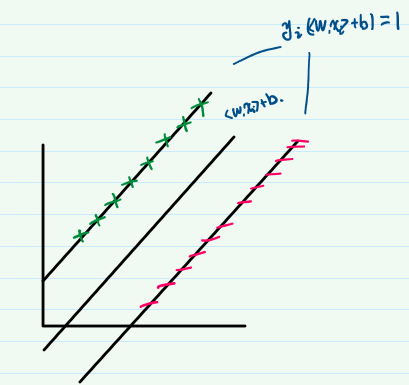
\includegraphics[width=0.5\textwidth]{caricature.png}
  \caption{Caricature of Data points}
  \end{figure}
  \color{orange}
  The parameter vector solution to the SVM problems can be written as:
  $$
  \wv = -\frac{1}{2} \xv_{1999} + \frac{1}{2} \xv_{1998}
  $$
  So only two points are required (i.e., only two points are the support vectors)\\

  The hard-margin SVM will have some issues with the dataset B. It runs forever. 
  This is because that the data points in dataset B are not linearly seperable, resulting the hard-margin SVM never halt. 
  We can also tell that these data points are not linearly seperable by the fact that the logistic regression succeeded. 
  Since if they are linearly seperable, that means perfect seperation and logistic regression will complain. 

  192 points are used to express the parameter vector as a linear combination of them. These points are the support vectors. 
  I got this result by calling soft\_svc.support\_ to get the list of indices of all support vectors, then count the length of this list.
  As for the accuracy, there are 57 wrong predictions for the soft-margin SVC method and 571 wrong predictions for the logistic regression method, 
  so the test loss for soft-margin SVC is around 0.0285 and for logistic regression is around 0.2855.
}

\item (Optional -- 0 pts) Construct a dataset in which every point is a support vector. 
  Do this for the soft margin ($C = 1$) and hard margin ($C = \infty$) cases.
  Make sure this dataset has $n \geq 100$ points.
  Submit these datasets in the \texttt{data} folder, as well as code required to generate them and demonstrate the number of support vectors.

    \ans{}

\end{enumerate}
\end{exercise}


\begin{exercise}[Support Vector Regression (8 pts)]
Let us consider support vector regression:
\begin{align}
\label{eq:CSVM}
\min_{\wv\in \RR^d, 
b\in\RR}  ~ \frac{1}{2} \|\wv\|_2^2 + C\sum_{i=1}^n \max\{ | y_i -  (\wv^\top \xv_i + b)| -\varepsilon , 0 \},
\end{align}
where $\xv_i \in \RR^d$, $y_i \in \RR$, and $\|\wv\|_2 := \sqrt{\sum_{j=1}^d w_j^2}$ is the Euclidean norm.
The above expression is the loss function, the error is simply the latter term $C\sum_{i=1}^n \max\{ | y_i -  (\wv^\top \xv_i + b)| -\varepsilon , 0 \}$.

\begin{enumerate}
	
\item (2 pts) Derive the Lagrangian dual of the support vector regression loss function \eqref{eq:CSVM}. Please include intermediate steps so that you can get partial credit.

\ans{
  We can rewrite the loss function as:
  $$
  \min_{\wv\in \RR^d, 
b\in\RR}  ~ \frac{1}{2} \|\wv\|_2^2 + C\sum_{i=1}^n \max\{ y_i -  (\wv^\top \xv_i + b) -\varepsilon, \wv^\top \xv_i + b - y_i -\varepsilon,  0 \}
  $$
  to get rid of the absolute value. Then, we can introduce a slack variable $\gamma_i$:
  $$
  \min_{\wv\in \RR^d, 
b\in\RR, \gamma in \RR^n}  ~ \frac{1}{2} \|\wv\|_2^2 + C\sum_{i=1}^n \gamma_i  \text{ s.t. } \gamma_i \ge y_i -  (\wv^\top \xv_i + b) -\varepsilon
  \text{ and } \gamma_i \ge \wv^\top \xv_i + b - y_i -\varepsilon
  \text{ and } \gamma_i \ge 0 \; \forall i
  $$
  Then we introduce dual variables and take Lagrangian:
    $$
  \max_{\alpha_i, \beta_i, \tau_i\in \RR^n, 
\alpha_i, \beta_i, \tau_i \ge 0}\min_{\wv, 
b, \gamma}  ~ \frac{1}{2} \|\wv\|_2^2 + \sum_{i=1}^n (C\gamma_i + \alpha_i (y_i -(\wv^\top \xv_i + b)-\varepsilon - \gamma_i) + 
\beta_i (\wv^\top \xv_i + b - y_i -\varepsilon - \gamma_i) - \tau_i\gamma_i)
  $$
  Then, let us take the derivative of this expression with respect to each variable and set them to zero:
  \begin{align*}
  F &= \frac{1}{2} \|\wv\|_2^2 + \sum_{i=1}^n (C\gamma_i + \alpha_i (y_i -(\wv^\top \xv_i + b)-\varepsilon - \gamma_i) + 
\beta_i (\wv^\top \xv_i + b - y_i -\varepsilon - \gamma_i) - \tau_i\gamma_i) \\
  \frac{\partial{F}}{\partial{\wv}} &= \wv + \sum_{i=1}^{n} \left(\frac{\partial}{\partial{\wv}} \left(-\alpha_i\wv^\top \xv_i + \beta_i \wv^\top \xv_i\right)\right)
            = \wv - \sum_{i=1}^{n} (\alpha_i - \beta_i) \xv_i = 0 \\
  \frac{\partial{F}}{\partial{b}} &= \sum_{i=1}^{n} \left(\frac{\partial}{\partial{b}} \left(-\alpha_i b + \beta_i b\right)\right)
            = \sum_{i=1}^{n} (-\alpha_i + \beta_i) = 0 \\  
  \frac{\partial{F}}{\partial{\gamma_i}} &= \frac{\partial}{\partial{\gamma_i}} \sum_{j=1}^{n} \left(C \gamma_j - \alpha_j \gamma_j - \beta_j \gamma_j - \tau_j \gamma_j\right)
            = C - \alpha_i - \beta_i - \tau_i = 0 \\  
  \end{align*}
  Then we can simplify the expression further with the result above:
  \begin{align*}
    F &= \frac{1}{2} \|\wv\|_2^2 + \sum_{i=1}^n (C - \alpha_i - \beta_i - \tau_i)\gamma_i
    + \sum_{i=1}^n (\alpha_i -\beta_i) y_i + \sum_{i=1}^n (- \alpha_i - \beta_i)\varepsilon + \sum_{i=1}^n (- \alpha_i + \beta_i)b + \sum_{i=1}^n (- \alpha_i + \beta_i)\wv^\top\xv_i \\
    &= \frac{1}{2} \|\wv\|_2^2 + \sum_{i=1}^n 0\gamma_i
    + \sum_{i=1}^n (\alpha_i -\beta_i) y_i - \varepsilon\sum_{i=1}^n (\alpha_i + \beta_i) + b\sum_{i=1}^n (- \alpha_i + \beta_i) - \sum_{i=1}^n (\alpha_i - \beta_i)\wv^\top\xv_i \\
    &= \frac{1}{2} \left\| \sum_{i=1}^{n} (\alpha_i - \beta_i) \xv_i \right\|_2^2 + \sum_{i=1}^n (\alpha_i -\beta_i) y_i - 2\varepsilon\sum_{i=1}^n \alpha_i - \sum_{i=1}^n (\alpha_i - \beta_i)\left(\sum_{j=1}^{n} (\alpha_j - \beta_j) \xv_j\right)^\top\xv_i \\
    &= \frac{1}{2} \left\| \sum_{i=1}^{n} (\alpha_i - \beta_i) \xv_i \right\|_2^2 + \sum_{i=1}^n (\alpha_i -\beta_i) y_i - 2\varepsilon\sum_{i=1}^n \alpha_i - \left(\sum_{j=1}^{n} (\alpha_j - \beta_j) \xv_j\right)^\top \sum_{i=1}^n (\alpha_i - \beta_i)\xv_i \\
    &= \frac{1}{2} \left\| \sum_{i=1}^{n} (\alpha_i - \beta_i) \xv_i \right\|_2^2 + \sum_{i=1}^n (\alpha_i -\beta_i) y_i - 2\varepsilon\sum_{i=1}^n \alpha_i - \left\| \sum_{i=1}^{n} (\alpha_i - \beta_i) \xv_i \right\|_2^2 \\
    &= -\frac{1}{2} \left\| \sum_{i=1}^{n} (\alpha_i - \beta_i) \xv_i \right\|_2^2 + \sum_{i=1}^n (\alpha_i -\beta_i) y_i - 2\varepsilon\sum_{i=1}^n \alpha_i \\
  \end{align*}
  \color{orange}
  So the problem is simplified to:
  \begin{align*}
    \max_{\alpha_i, \beta_i, \tau_i\in \RR^n, \alpha_i, \beta_i, \tau_i \ge 0} -\frac{1}{2} \left\| \sum_{i=1}^{n} (\alpha_i - \beta_i) \xv_i \right\|_2^2 + \sum_{i=1}^n (\alpha_i -\beta_i) y_i - 2\varepsilon\sum_{i=1}^n \alpha_i \\
    \text{ s.t } \sum_{i=1}^{n} (-\alpha_i + \beta_i) = 0 \text{ and } C - \alpha_i - \beta_i - \tau_i = 0
  \end{align*}
  We can further simplified this by eliminating $\tau_i$ because $\tau_i = C - \alpha_i - \beta_i \ge 0$ to get:
  \begin{align*}
    \max_{\alpha_i, \beta_i \in \RR^n, \alpha_i, \beta_i \ge 0, C \ge \alpha_i + \beta_i} -\frac{1}{2} \left\| \sum_{i=1}^{n} (\alpha_i - \beta_i) \xv_i \right\|_2^2 + \sum_{i=1}^n (\alpha_i -\beta_i) y_i - 2\varepsilon\sum_{i=1}^n \alpha_i \\
    \text{ s.t } \sum_{i=1}^{n} (-\alpha_i + \beta_i) = 0
  \end{align*}
  or 
  \begin{align*}
    \min_{\alpha_i, \beta_i \in \RR^n, \alpha_i, \beta_i \ge 0, C \ge \alpha_i + \beta_i} \frac{1}{2} \left\| \sum_{i=1}^{n} (\alpha_i - \beta_i) \xv_i \right\|_2^2 - \sum_{i=1}^n (\alpha_i -\beta_i) y_i + 2\varepsilon\sum_{i=1}^n \alpha_i \\
    \text{ s.t } \sum_{i=1}^{n} (-\alpha_i + \beta_i) = 0
  \end{align*}
} 


\vskip1cm

In the following you will complete and implement the following gradient algorithm for solving support vector regression in \Cref{eq:CSVM}:

\begin{algorithm}[H]
	\DontPrintSemicolon
	\KwIn{$X\in\RR^{n\times d}$, $\yv\in \RR^n$, $\wv=\zero_d$, $b=0$, $\mathsf{max\_pass} \in \mathds{N}$, step size $\eta$}
	
	\KwOut{$\wv, b$}
	
	\For{$t=1, 2, \ldots, \mathsf{max\_pass}$ }{
		
		\For{$i=1, 2, \ldots, n$}{
			
			choose step size $\eta$
			
			\If{$|y_i - (\inner{\xv_i}{\wv}+b)| \geq \varepsilon$}{
				$\wv \gets $ \tcp*{$\xv_i$ is the $i$-th row of $X$}
				
				$b \gets $
			}	
			
			$\wv \gets $ \tcp*{proximal step}
		}
	}
	\caption{GD for SVR.}
	\label{alg:CSVM}
\end{algorithm}

    Note that this differs a bit from what you've seen so far, in terms of gradient descent. Rather than taking steps based on the entire loss function, we instead take a step based on the unregularized loss, and then perform a projection step based on the regularizer (sometimes called a ``proximal step'').

\item (2 pts) Compute the gradient with respect to $\wv$ and $b$ for each second term in \Cref{eq:CSVM}.
Note that in places where the function is non-differentiable, you might have to compute a sub-gradient.
\begin{align}
C\sum_{i=1}^n \max\{ | y_i -  (\wv^\top \xv_i + b)| -\varepsilon , 0 \}
\end{align}
	
	
\ans{
  Take the loss function in an equivalent form as:
  \begin{align*}
    L = C\sum_{i=1}^n \max\{y_i - \wv^\top \xv_i - b - \varepsilon, \wv^\top \xv_i + b - y_i -\varepsilon , 0 \}
  \end{align*}
  \color{orange}
  We can calculate the gradient of each expression inside the max:
  \begin{align*}
    \frac{\partial}{\partial{\wv}} y_i - \wv^\top \xv_i - b - \varepsilon &= -\xv_i \\
    \frac{\partial}{\partial{\wv}} \wv^\top \xv_i + b - y_i - \varepsilon &= \xv_i \\
    \frac{\partial}{\partial{\wv}} 0 &= 0 \\
  \end{align*}
  The gradient can be expressed as:
  \begin{align*}
    \frac{\partial{L}}{\partial{\wv}} = C\sum_{i=1}^n \varsigma_i \quad
    \frac{\partial{L}}{\partial{d}} = C\sum_{i=1}^n \sigma_i
  \end{align*}
  where $\varsigma_i$ is:
  \begin{align*}
    \varsigma_i = \left\{
        \begin{array}{ll}
            -\xv_i & \quad y_i \ge \wv^\top \xv_i + b \text{ and }  y_i - \wv^\top \xv_i - b - \varepsilon \ge 0 \\
            \xv_i & \quad  y_i \le \wv^\top \xv_i + b \text{ and }  \wv^\top \xv_i + b - y_i - \varepsilon \ge 0 \\
            0 & \quad y_i - \wv^\top \xv_i - b - \varepsilon \le 0 \text{ and }  \wv^\top \xv_i + b - y_i - \varepsilon \le 0\\
        \end{array}
    \right. \\
    \sigma_i = \left\{
        \begin{array}{ll}
            -1 & \quad y_i \ge \wv^\top \xv_i + b \text{ and }  y_i - \wv^\top \xv_i - b - \varepsilon \ge 0 \\
            1 & \quad  y_i \le \wv^\top \xv_i + b \text{ and }  \wv^\top \xv_i + b - y_i - \varepsilon \ge 0 \\
            0 & \quad y_i - \wv^\top \xv_i - b - \varepsilon \le 0 \text{ and }  \wv^\top \xv_i + b - y_i - \varepsilon \le 0\\
        \end{array}
    \right.
  \end{align*}
  we can simplify this a little bit if we consider that $\varepsilon \ge 0$:
    \begin{align*}
    \varsigma_i = \left\{
        \begin{array}{ll}
            -\xv_i & \quad y_i - (\wv^\top \xv_i + b ) \ge \varepsilon \\
            \xv_i & \quad  y_i - (\wv^\top \xv_i + b ) \le -\varepsilon\\
            0 & \quad  - \varepsilon \le y_i - (\wv^\top \xv_i + b ) \le \epsilon\\
        \end{array}
    \right. \\
    \sigma_i = \left\{
        \begin{array}{ll}
            -1 & \quad y_i - (\wv^\top \xv_i + b ) \ge \varepsilon \\
            1 & \quad  y_i - (\wv^\top \xv_i + b ) \le -\varepsilon\\
            0 & \quad  - \varepsilon \le y_i - (\wv^\top \xv_i + b ) \le \epsilon\\
        \end{array}
    \right.
  \end{align*}
} 

	
\item (1 pt) Find the closed-form solution of the following proximal step:
	\begin{align}
	\mathsf{P}^\eta(\wv) = \argmin_{\zv} ~ \frac{1}{2\eta} \|\zv - \wv\|_2^2 + \frac{1}{2} \|\zv\|_2^2
	\end{align}
	
	
\ans{
  To find the mininum value, we take the derivatives of this expression:
  \begin{align*}
    \frac{\partial}{\partial{\zv}} \left(\frac{1}{2\eta} \|\zv - \wv\|_2^2 + \frac{1}{2} \|\zv\|_2^2\right) 
    &= \zv + \frac{1}{\eta} (\zv - \wv) \\
     \frac{\partial^2}{\partial{\wv^2}} \left(\frac{1}{2\eta} \|\zv - \wv\|_2^2 + \frac{1}{2} \|\zv\|_2^2\right) 
    &= \frac{\partial}{\partial{\wv}} \left(\zv + \frac{1}{\eta} (\zv - \wv) \right)\\
    &= 1 + \frac{1}{\eta} > 0\\
  \end{align*}
  The second derivative about $\zv$ is positive, so the expression is convex. Therefore, the expression will take \\
  its minimum at the point when we set the first derivative to zero.
  \color{orange}
  \begin{align*}
    \zv + \frac{1}{\eta} (\zv - \wv) &= 0\\
    \eta \zv + \zv - \wv &= 0 \\
    \zv &= \frac{\wv}{1+\eta}
  \end{align*}
  Therefore:
  \begin{align}
	\mathsf{P}^\eta(\wv) = \frac{\wv}{1+\eta}
	\end{align}
} 

	
\item (3 pts) Implement \Cref{alg:CSVM}. You should use part 2 to complete lines 5-6, and part 3 for line 7. 
Run it on Mystery Dataset C (this is Mystery Dataset A from Assignment 1, but reused), and report your training error, training loss, and test error. Use $C=1$ and $\varepsilon = 0.5$.

\ans{
  Please see the implementation in the script file. The report is: \\
  training error: 610.2011152463025 \\
  training loss: 610.7272490389753 \\
  test error: 775.7902535073246
} 

\end{enumerate}
\end{exercise}

\begin{exercise}[Kernels (5 pts)]
      For the following questions you might find it useful to recall the definition of a matrix being positive semidefinite (PSD).
      A matrix $M \in \mathbb{R}^{d \times d}$ is PSD if and only if $x^T Mx \geq 0$ for all vectors $x \in \mathbb{R}^d$.
      It may also be helpful to refresh yourself on Taylor series.

  \begin{enumerate}
    \item (2 pt) For $x, y \in \mathbb{R}$, consider the kernel function $k(x, y) = \exp\left(-\alpha\left(x - y\right)^2\right)$.
      What is the corresponding feature map $\phi(\cdot)$ such that $\phi(x)^T \phi(y) = k(x, y)$?
      If you were using this kernel for an SVM model, would you prefer to solve the primal or dual representation? Why?

\ans{
  The corresponding feature map is:
  \begin{align*}
  \phi(x) &= e^{-\alpha x^2} [1, \sqrt{\frac{1}{1!}}(-\sqrt{2\alpha}x), \sqrt{\frac{1}{2!}}(-\sqrt{2\alpha}x)^2, \cdots]^T \\
  &= e^{-\alpha x^2} v^T 
  \end{align*}
  where $v^\top$ is a $\mathbb{R}^{\infty}$ vector and $v_1 = 1$, $v_i = \sqrt{\frac{1}{(i-1)!}}(-\sqrt{2\alpha}x)^{i-1}$ for all other $i$. \\
  I prefer solve the dual because we only need to consider about the dot product, or the kernel in the dual representation. Since $\phi(x)$ 
  will be a vector with infinite size, calculating the vector itself will be really expensive in the primal representation.
}


    \item (1 pt) Consider the function $\frac{1}{1 - xy}$, where $x, y \in (-1, 1)$.
      Is this function a valid kernel?
      If so, write out the corresponding feature map $\phi(\cdot)$, if not, explain why.

\ans{
  This function is a valid kernel. The feature map is:
  \begin{align*}
  \phi(x) &= [1, x, x^2, x^3, \cdots]^\top \\
  &= v^\top
  \end{align*}
  where $v^\top$ is a $\mathbb{R}^{\infty}$ vector and $v_i = x^{i-1}$ for all integer $i=1,2,3,\cdots$.
}
    \item (1 pt) Consider the function $\log (1 + xy)$, where $0 < x, y \in \mathbb{R}$.
      Is this function a valid kernel?
      If so, write out the corresponding feature map $\phi(\cdot)$, if not, explain why.

\ans{
  \color{orange}
  This is not a valid kernel. We can consider the dataset:
  $$
    x_1 = 1, y_1 = 2, x_2 = 2, y_2 = 1
  $$
  and
  $$
  v = [-1, 1]^\top
  $$
  So the kernel will be:
  $$
  K = \begin{bmatrix}
        \log(3) & \log(2) \\
        \log(5) & \log(3)
        \end{bmatrix}
  $$
  Therefore:
  \begin{align*}
    v^\top K v &= [-1, 1] \begin{bmatrix}
        \log(3) & \log(2) \\
        \log(5) & \log(3)
        \end{bmatrix} \begin{bmatrix}
        -1 \\
        1 
        \end{bmatrix} \\
        &= [-\log 3 + \log 5, -\log2 + \log3] \begin{bmatrix}
        -1 \\
        1 
        \end{bmatrix} \\
        &= \log3 - \log5 - \log2 + \log 3 \\
        & = \log(\frac{9}{10}) < 0
  \end{align*}
}
    \item (1 pt) Consider the function $\cos(x + y)$, where $x, y \in \mathbb{R}$.
      Is this function a valid kernel?
      If so, write out the corresponding feature map $\phi(\cdot)$, if not, explain why.

\ans{
  This is not a valid kernel. We can consider the dataset:
  $$
    x_1 = 0, y_1 = \frac{3\pi}{2}, x_2 = \frac{\pi}{2}, y_2 = 0
  $$
  and
  $$
  v = [-1, 1]^\top
  $$
  So the kernel will be:
  $$
  K = \begin{bmatrix}
        \cos(\frac{3\pi}{2}) & \cos(0) \\
        \cos(2\pi) & \frac{\pi}{2}
        \end{bmatrix}
    = \begin{bmatrix}
        0 & 1 \\
        1 & 0
        \end{bmatrix}
  $$
  Therefore:
  \begin{align*}
    v^\top K v &= [-1, 1] \begin{bmatrix}
        0 & 1 \\
        1 & 0
        \end{bmatrix}\begin{bmatrix}
        -1 \\
        1 
        \end{bmatrix} \\
        &= [1, -1] \begin{bmatrix}
        -1 \\
        1 
        \end{bmatrix} \\
        &= -2 < 0
  \end{align*}
}
  \end{enumerate}
\end{exercise}

\end{document}
              
